
\subsection{Rezultati testiranja stranice Blog}

\begin{figure}[H]
    \centering
    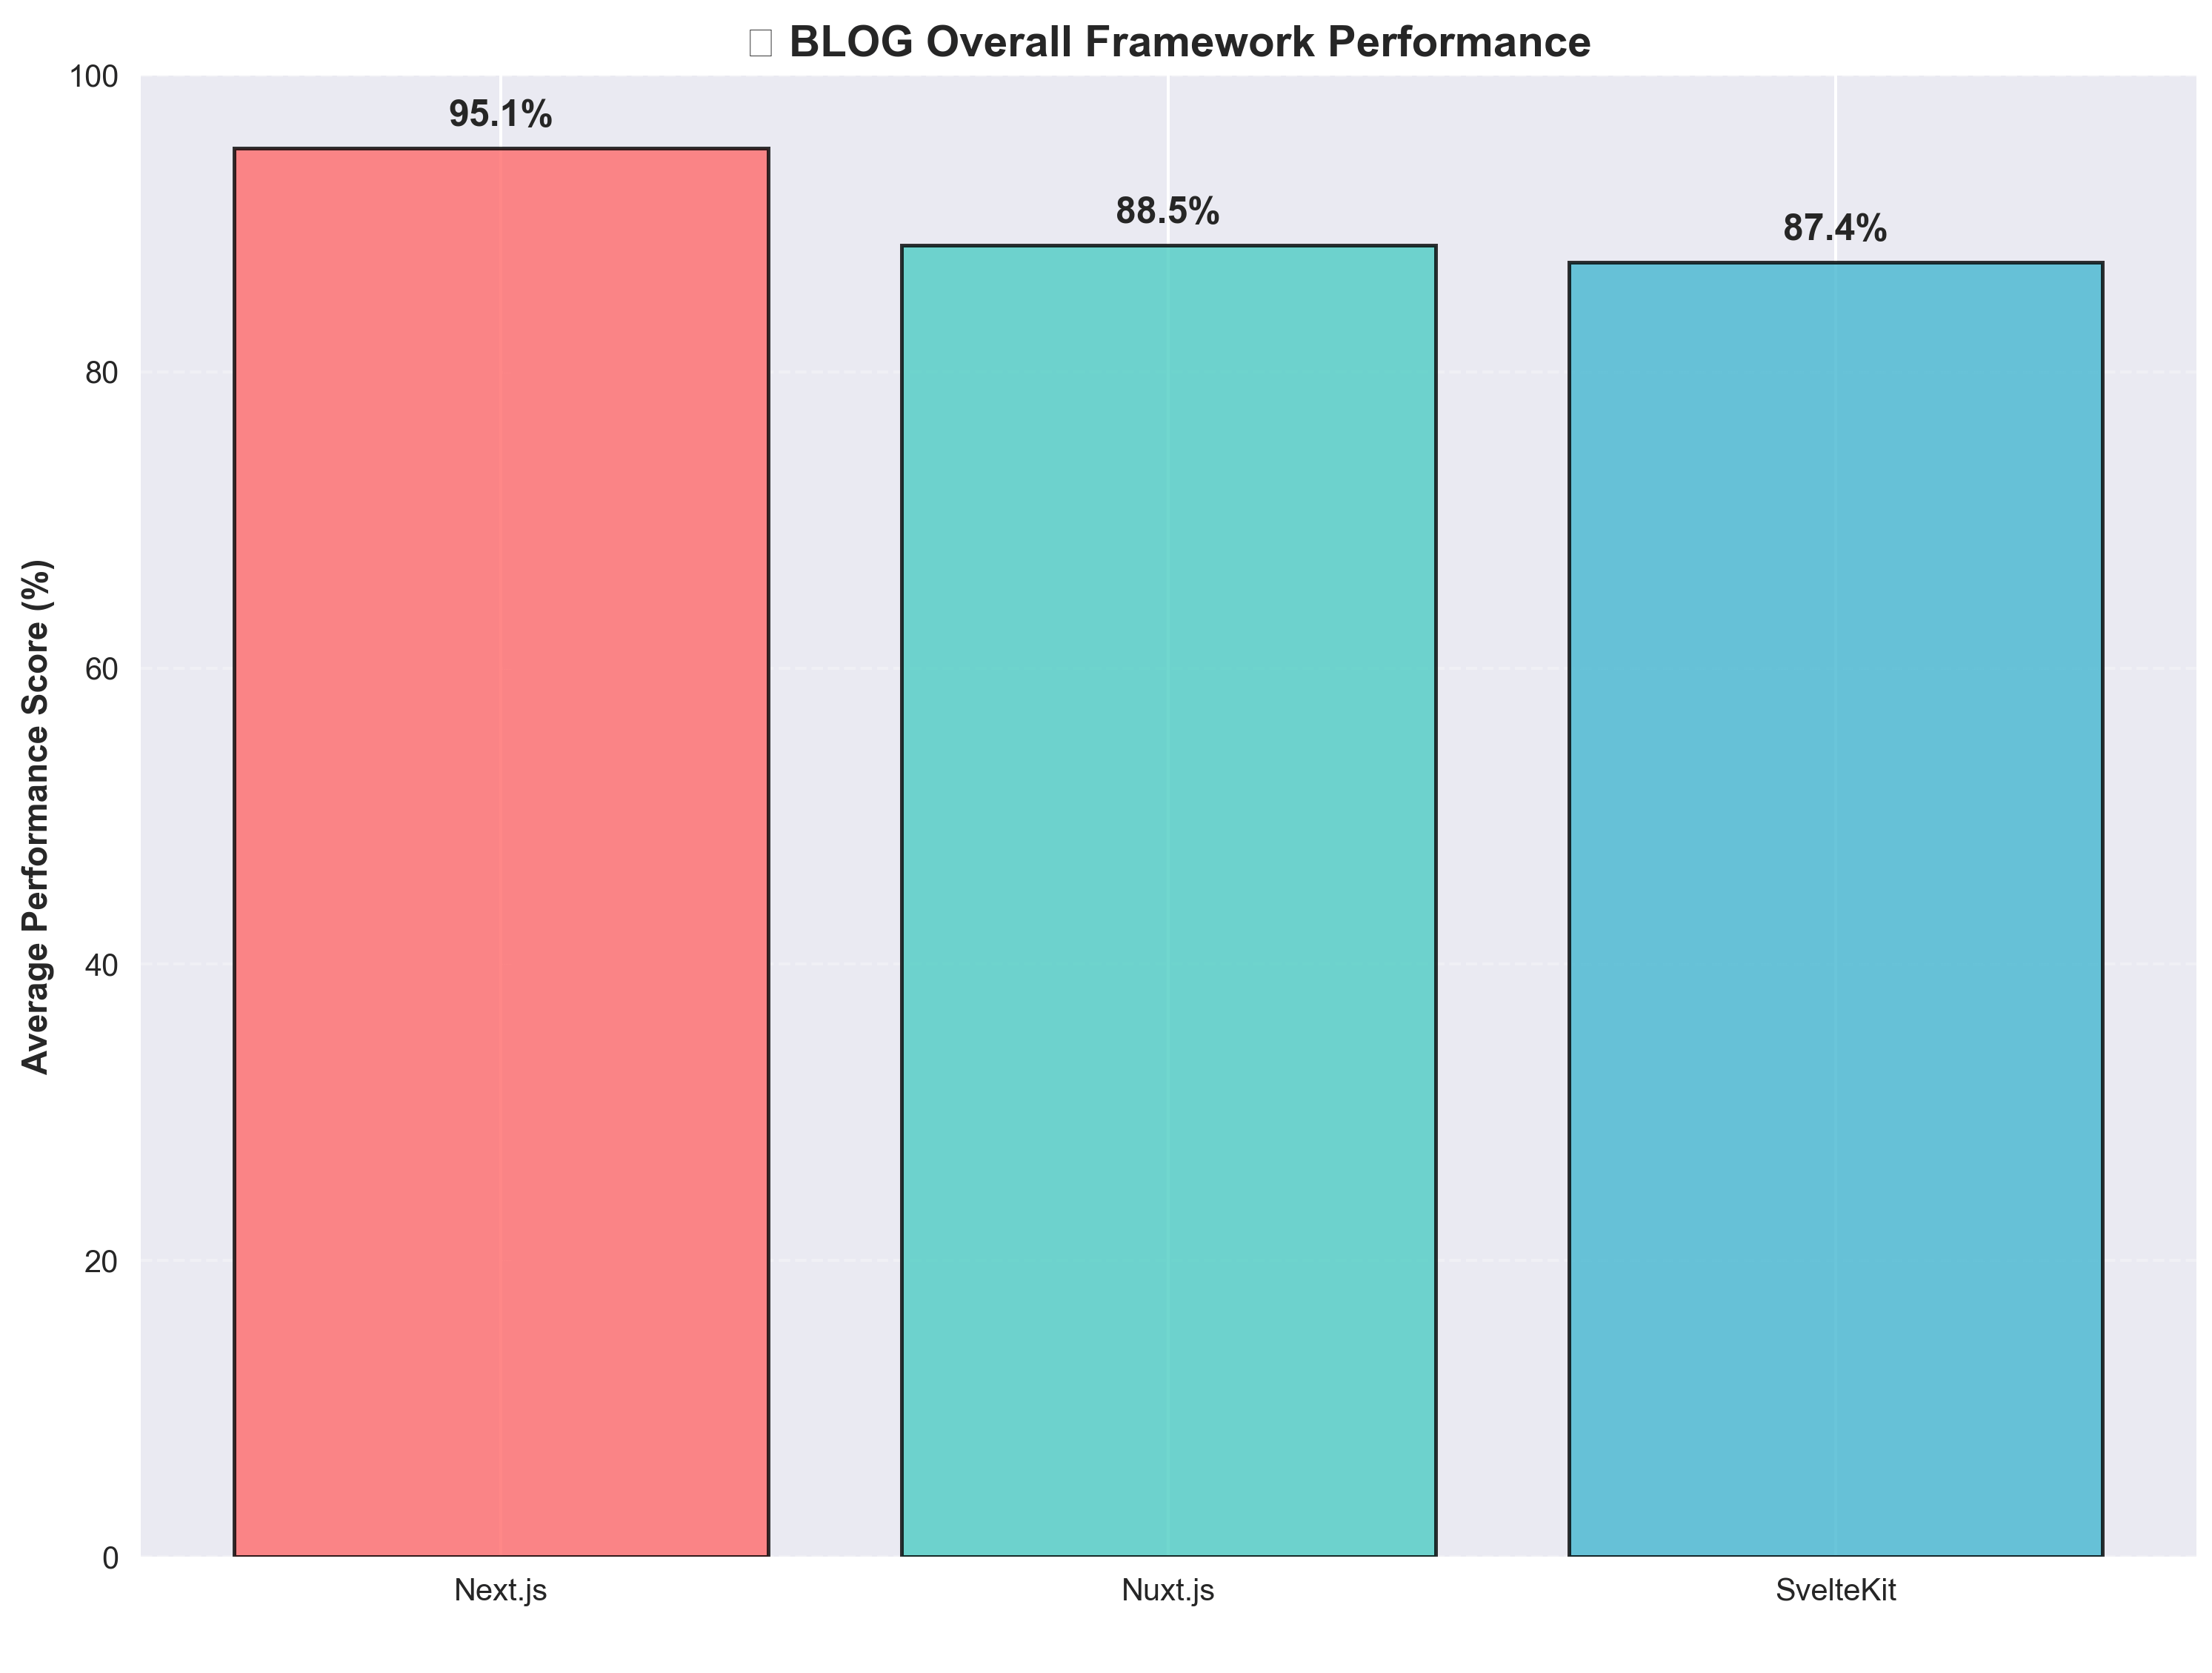
\includegraphics[width=0.8\textwidth]{slike/rezultati/blog/blog_framework_overall_performance.png}
    \caption{Ukupne ocjene radnih značajki (stranica Blog)}
    \label{fig:testiranje-blog-ukupne-performanse}
\end{figure}

\begin{figure}[H]
    \centering
    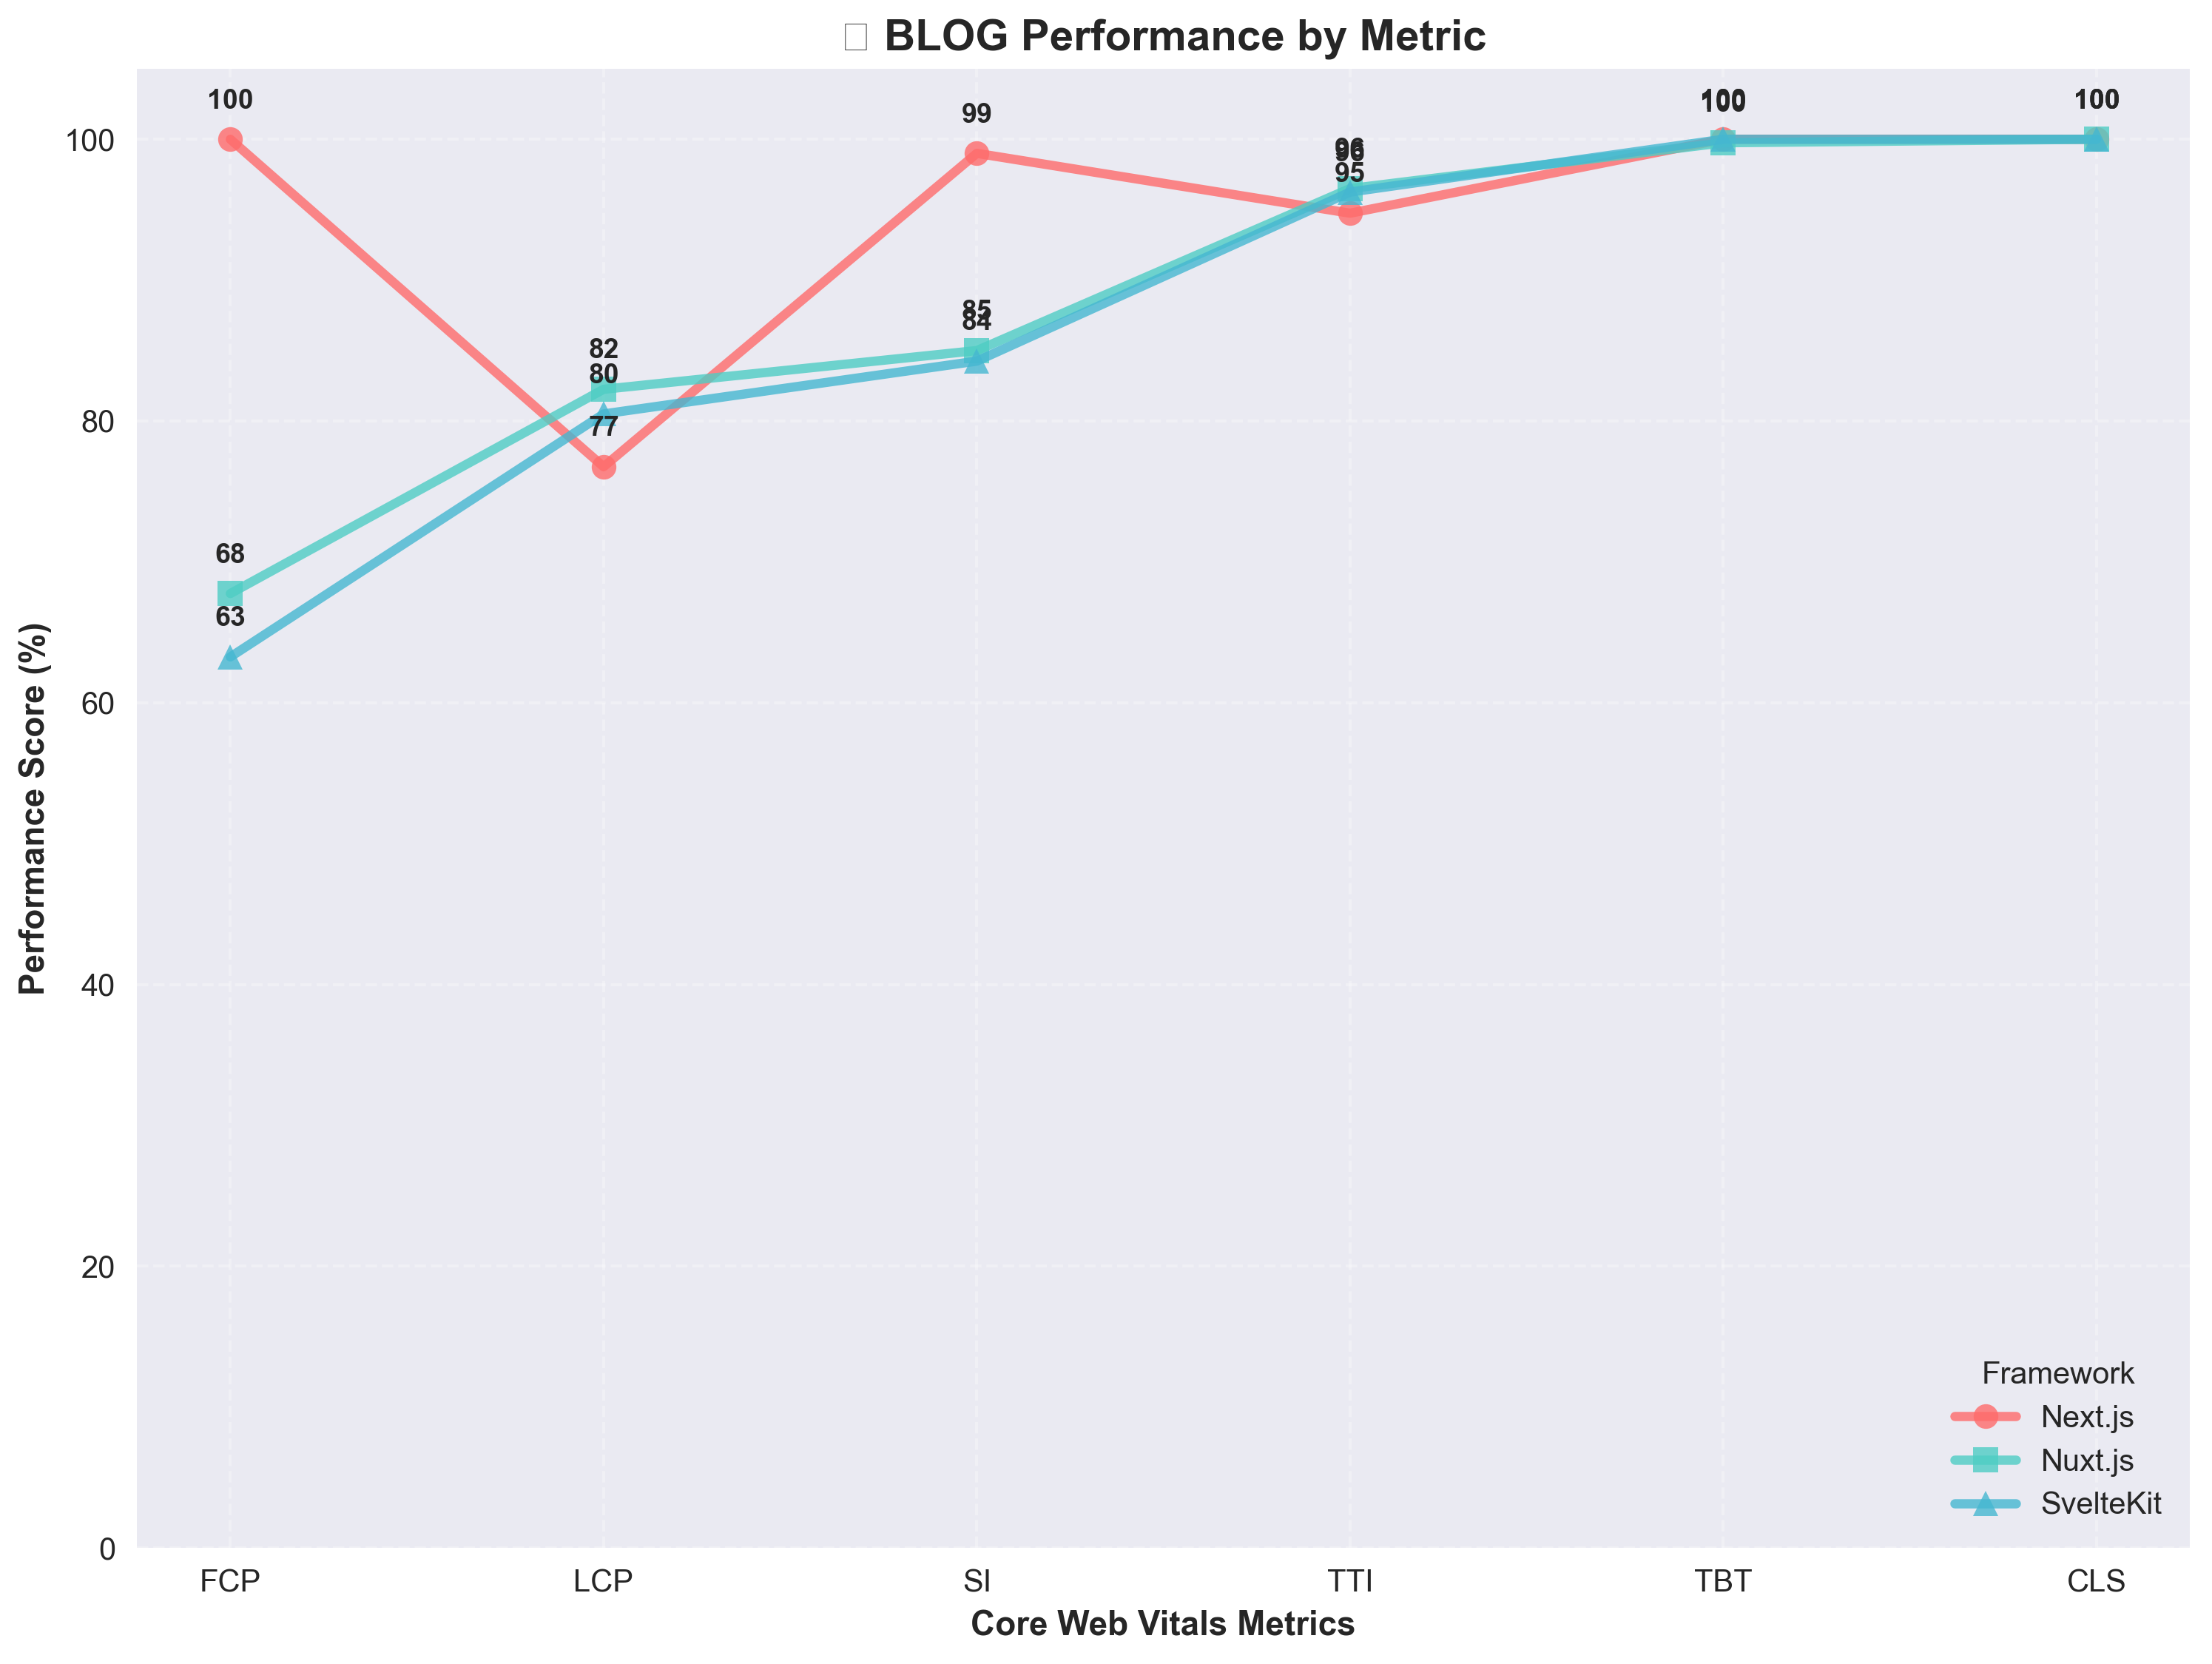
\includegraphics[width=0.8\textwidth]{slike/rezultati/blog/blog_performance_by_metric.png}
    \caption{Ukupne ocjene radnih značajki po metrici (stranica Blog)}
    \label{fig:testiranje-blog-performanse-po-metrici}
\end{figure}

\begin{figure}[H]
    \centering
    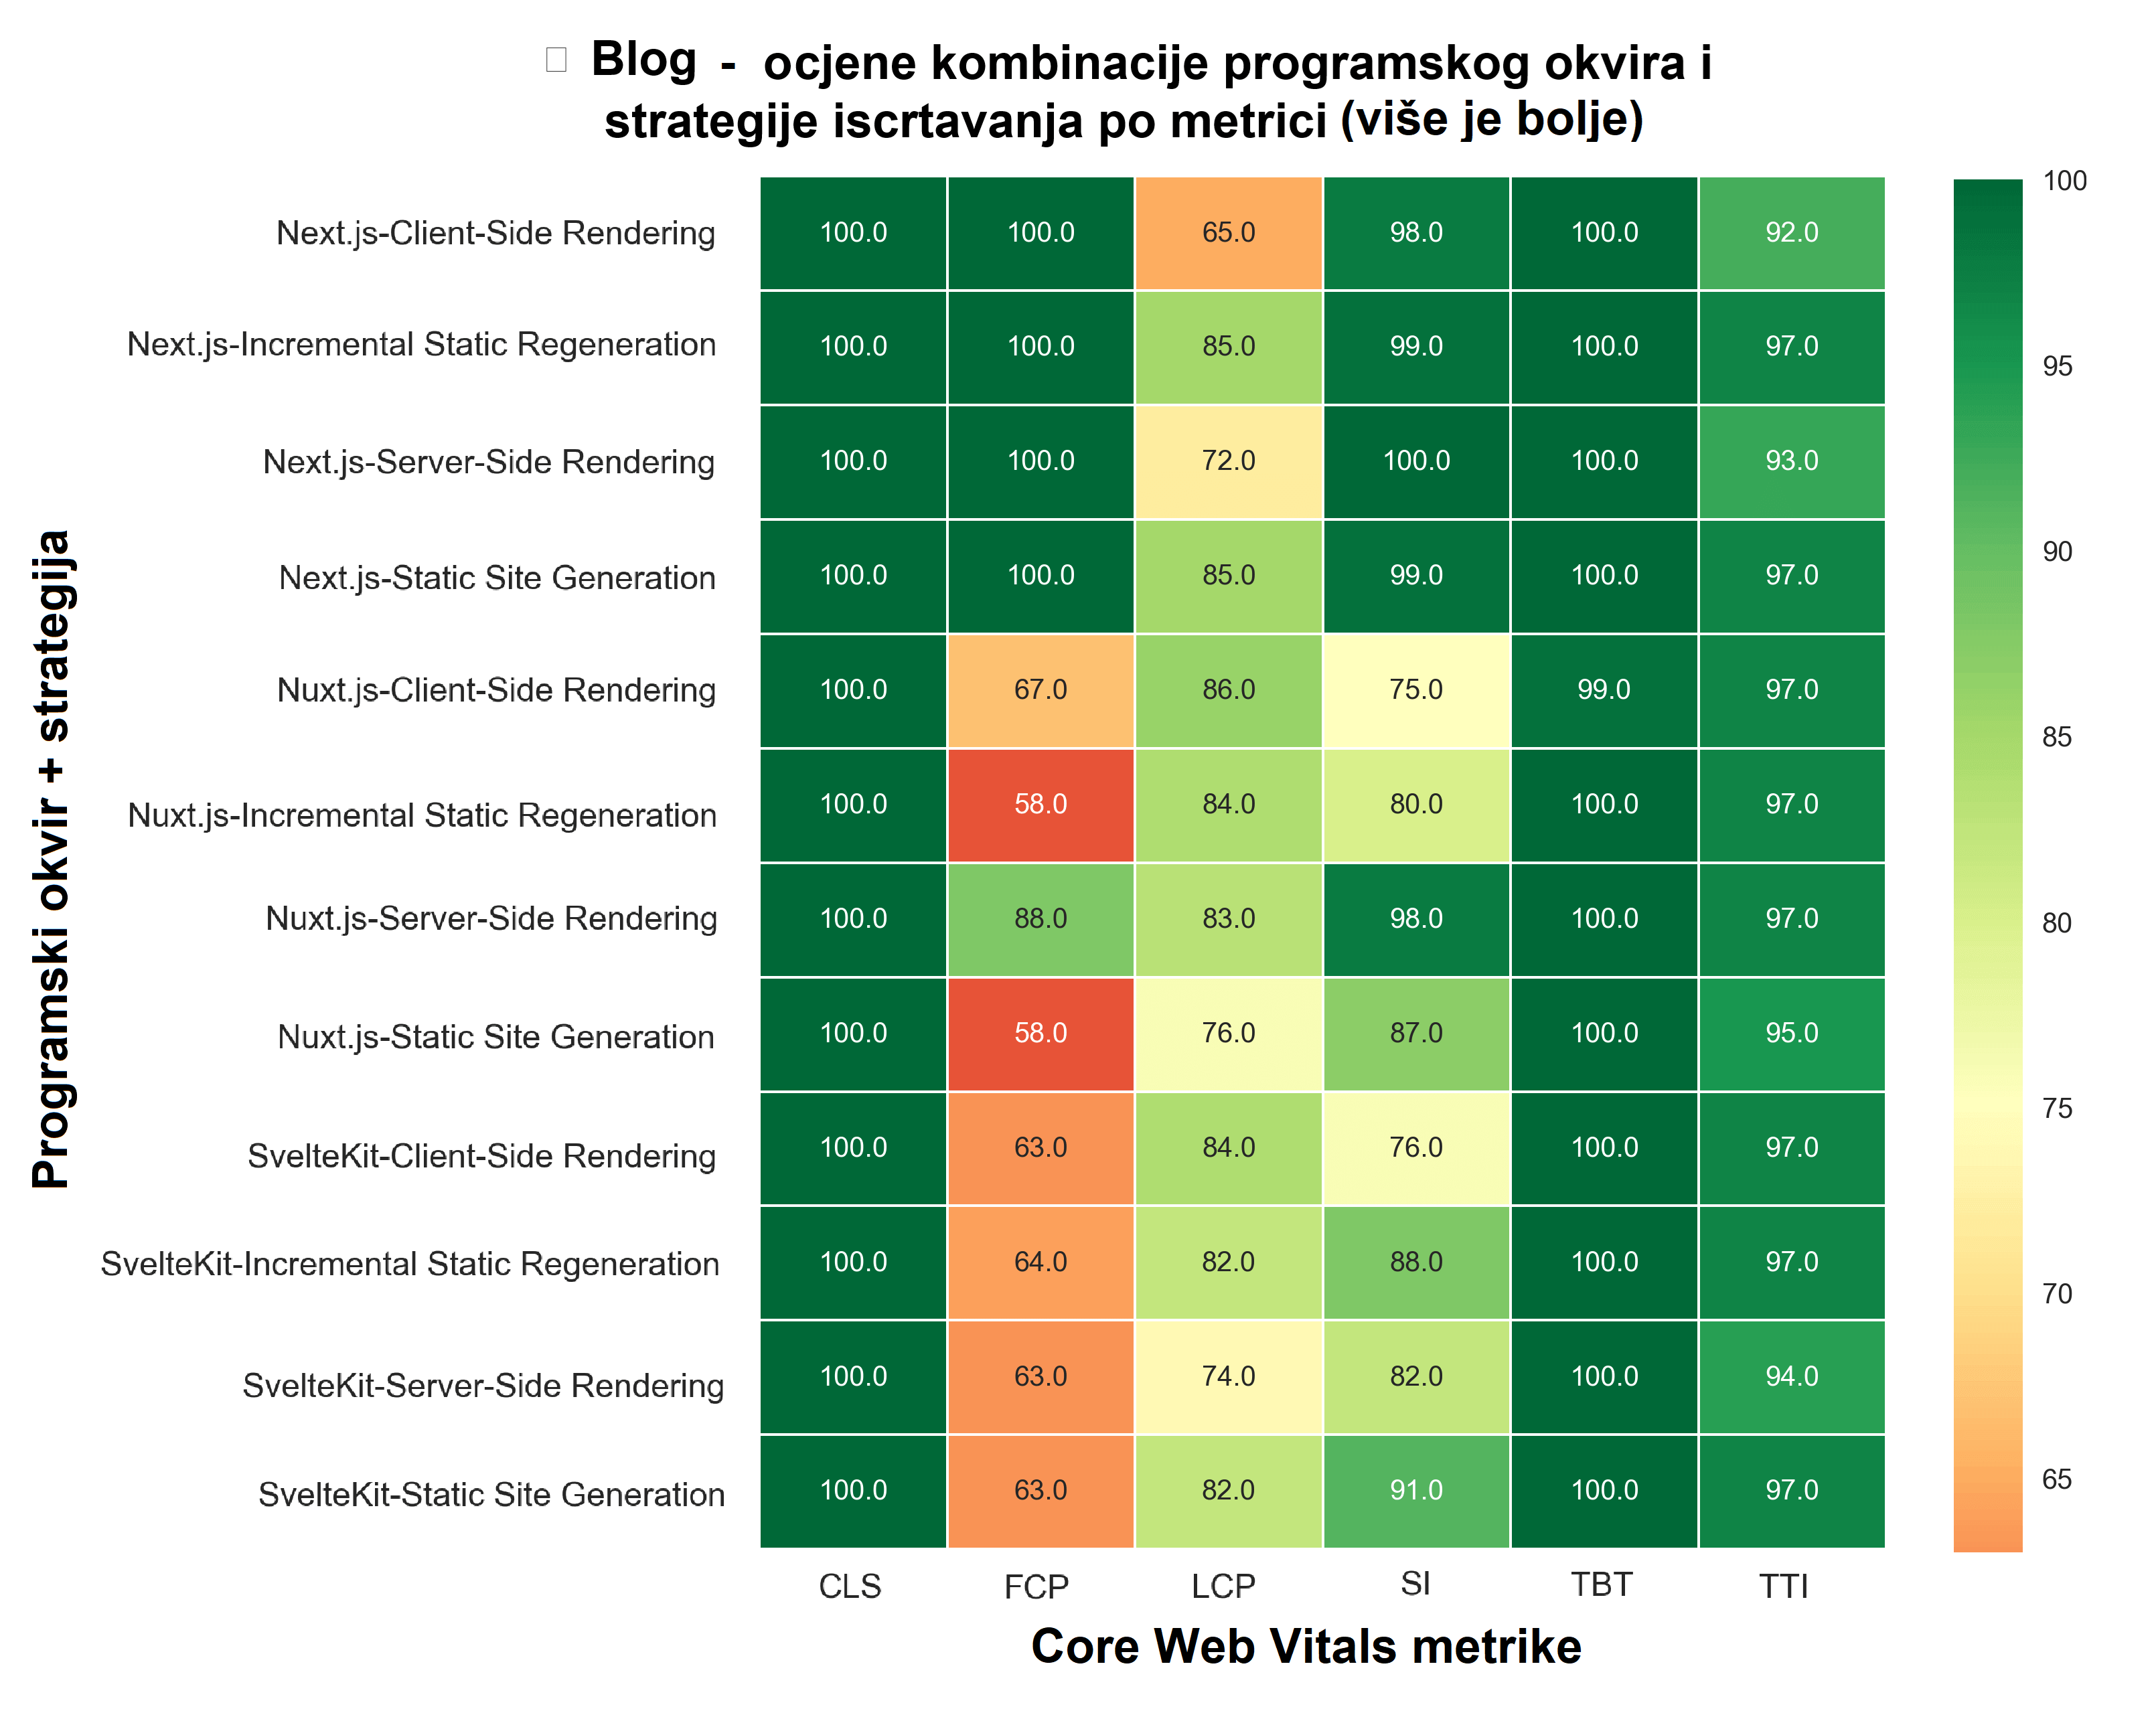
\includegraphics[width=\textwidth]{slike/rezultati/blog/blog_performance_scores.png}
    \caption{Ocjene radnih značajki - postotak (stranica Blog)}
    \label{fig:testiranje-blog-postotak}
\end{figure}

\begin{figure}[H]
    \centering
    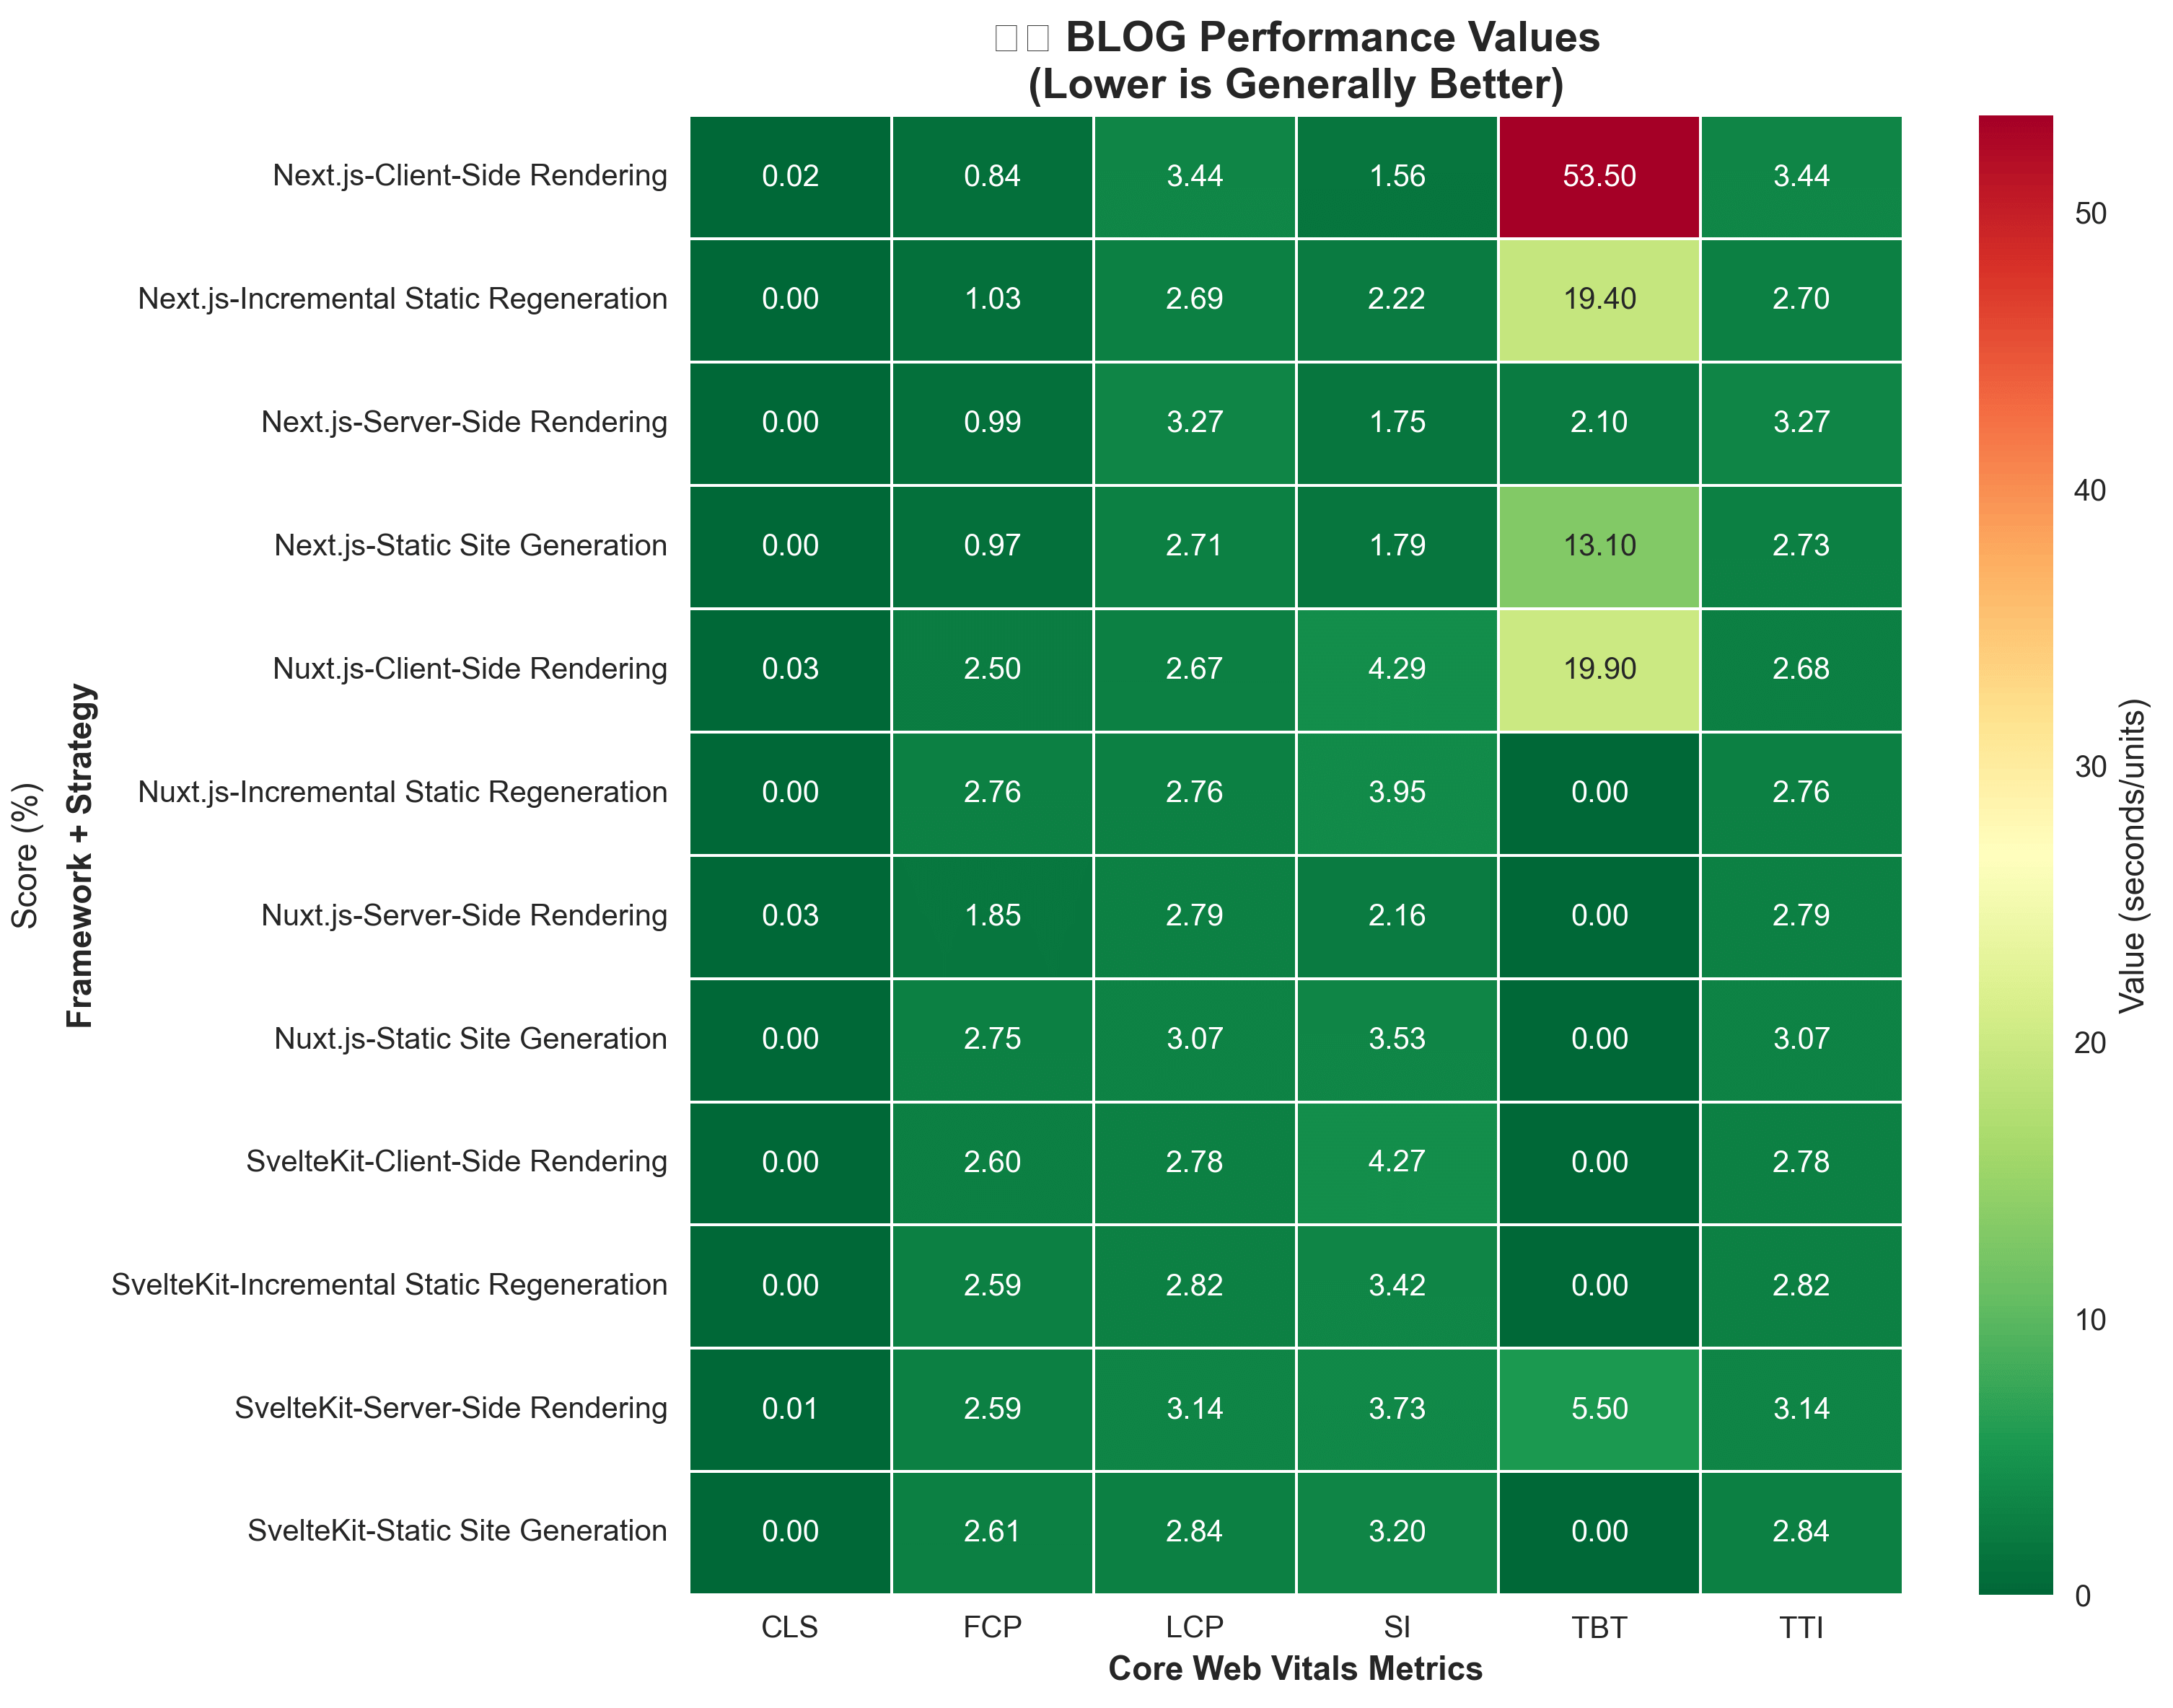
\includegraphics[width=\textwidth]{slike/rezultati/blog/blog_performance_values.png}
    \caption{Ocjene radnih značajki - vrijednosti (stranica Blog)}
    \label{fig:testiranje-blog-vrijednosti}
\end{figure}

\begin{figure}[H]
    \centering
    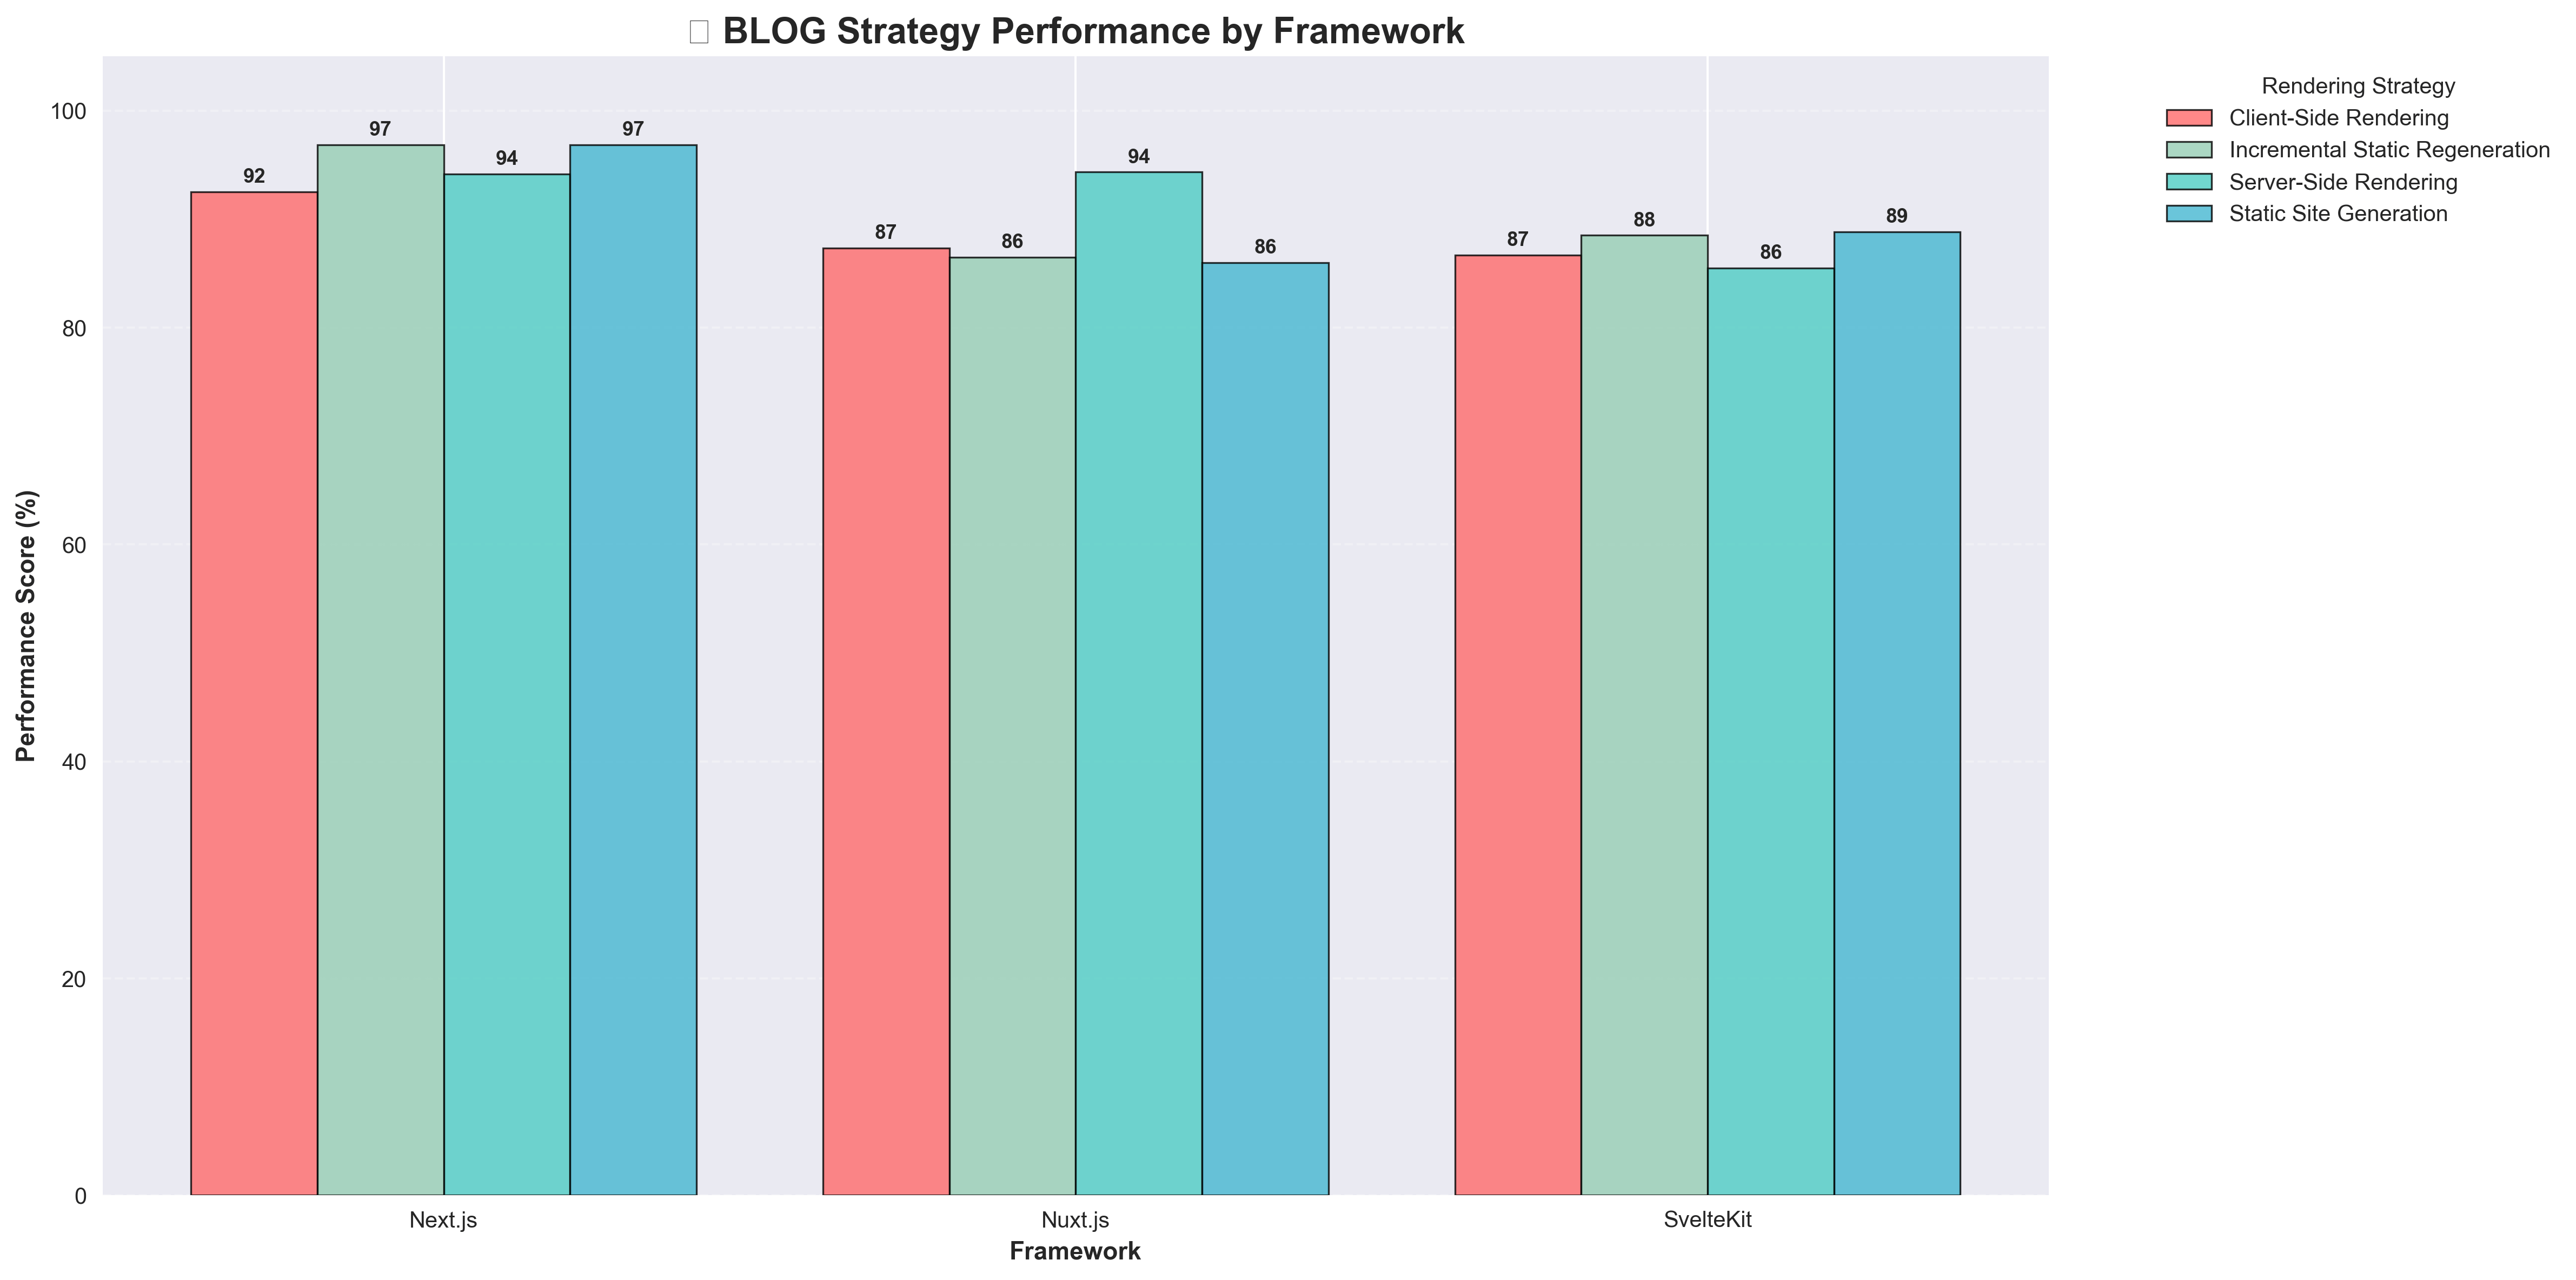
\includegraphics[width=\textwidth]{slike/rezultati/blog/blog_strategy_comparison.png}
    \caption{Ocjene radnih značajki - usporedba strategija (stranica Blog)}
    \label{fig:testiranje-blog-usporedba-strategija}
\end{figure}

\newpage

\subsection{Sažetak rezultata - stranica Blog}

\begin{table}[H]
    \centering
    \caption{Sažetak rezultata testiranja stranice Blog}
    \label{tab:sazetak-rezultata-blog}
    \renewcommand{\arraystretch}{1.5}
    \resizebox{\textwidth}{!}{%
        \begin{tabular}{|l|l|l|}
            \hline
            \textbf{Kategorija} & \textbf{Element}                             & \textbf{Ocjena}    \\
            \hline
            \multirow{3}{*}{\textbf{Programski okviri}}
                                & 1. Next.js                                   & 95.1\% (±9.4\%)   \\[0.2em]
                                & 2. Nuxt.js                                   & 88.5\% (±13.5\%)  \\[0.2em]
                                & 3. SvelteKit                                 & 87.4\% (±13.7\%)  \\
            \hline
            \multirow{4}{*}{\textbf{Strategije iscrtavanja}}
                                & 1. Server-Side Rendering                     & 91.3\% (±11.7\%)  \\[0.2em]
                                & 2. Incremental Static Regeneration           & 90.6\% (±12.9\%)  \\[0.2em]
                                & 3. Static Site Generation                    & 90.6\% (±13.2\%)  \\[0.2em]
                                & 4. Client-Side Rendering                     & 88.8\% (±13.7\%)  \\
            \hline
            \multirow{5}{*}{\textbf{Najbolje kombinacije}}
                                & 1. Next.js + Incremental Static Regeneration & 96.8\% (±5.9\%)   \\[0.2em]
                                & 2. Next.js + Static Site Generation          & 96.8\% (±5.9\%)   \\[0.2em]
                                & 3. Nuxt.js + Server-Side Rendering           & 94.3\% (±7.1\%)   \\[0.2em]
                                & 4. Next.js + Server-Side Rendering           & 94.2\% (±11.2\%)  \\[0.2em]
                                & 5. Next.js + Client-Side Rendering           & 92.5\% (±13.8\%)  \\
            \hline
            \multirow{6}{*}{\textbf{Vodeći po metrici}}
                                & FCP: Next.js + Client-Side Rendering         & 100.0\% (0.840s)   \\[0.2em]
                                & LCP: Nuxt.js + Client-Side Rendering         & 86.0\% (2.670s)    \\[0.2em]
                                & SI: Next.js + Server-Side Rendering          & 100.0\% (1.750s)   \\[0.2em]
                                & TTI: Nuxt.js + Client-Side Rendering         & 97.0\% (2.680s)    \\[0.2em]
                                & TBT: Next.js + Client-Side Rendering         & 100.0\% (53.500ms) \\[0.2em]
                                & CLS: Next.js + Client-Side Rendering         & 100.0\% (0.020)    \\
            \hline
        \end{tabular}%
    }
\end{table}

